\section{Analysis}
\label{sec:analysis}

% Edge inference was performed on a few different graphs where the true gold standard edges are known. Node values are then simulated using these known graphs using two different methods. The node values represent the RNA log fold-change values found experimentally. By inferring the edges using the simulated node values we evaluate the performance of edge inference. Lastly, the experimental yeast data is applied for edge inference for protein kinase interactions, while transcription factor interactions are assumed known.

\begin{frame}{Directed acyclic graph}
\label{sec:dag}
% Inference of edges was first tested as a proof-of-concept on a small DAG~(\autoref{fig:dag}). The DAG is designed with 3 protein kinases and 3 transcription factors, with a combination of positive and negative gene regulation control mediated by the TFs, as well as a combination of positive and negative protein activity regulation mediated by the PKs.
\begin{figure}[ht]
    \centering
    \includegraphics[width=0.3\textwidth]{analysis/fig/dag.pdf}
    \caption{\textbf{DAG example.} Pointed/closed arrowhead: edge value = 1, flat/open: -1. }
    \label{fig:dag}
\end{figure}
% As described in~\autoref{sec:equilibrium_model}, each of the six nodes are defined by observations of their simulated log fold-change RNA values as well as defined by their unobserved activity attribute.
Comparing
\begin{itemize}
    \item simple simulation vs. GNW extension
    \item $\boldsymbol{e}$-minimization vs. LLC
\end{itemize}
\end{frame}

\begin{frame}{Directed acyclic graph - simulation}
\begin{columns}
\begin{column}{0.2\textwidth}
Both simulation methods work intuitively
\end{column}
\begin{column}{0.8\textwidth}
\begin{figure}[ht]
\centering
\begin{subfigure}[b]{0.44\textwidth}\centering\caption{}
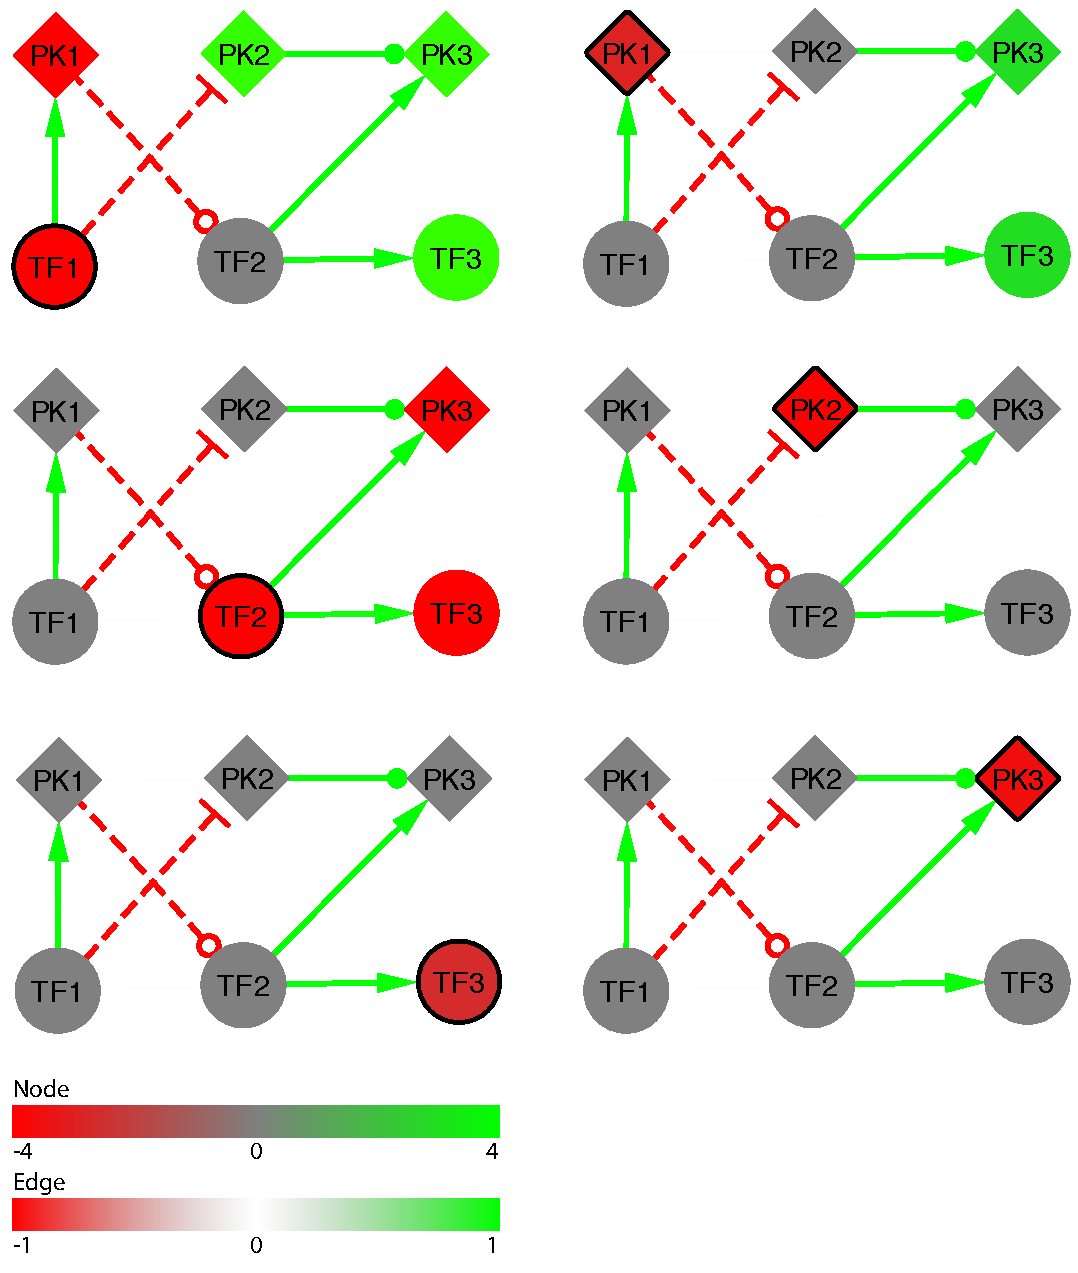
\includegraphics[width=\textwidth]{analysis/fig/prim.pdf}
\end{subfigure}
\hfill
\begin{subfigure}[b]{0.44\textwidth}\centering\caption{}
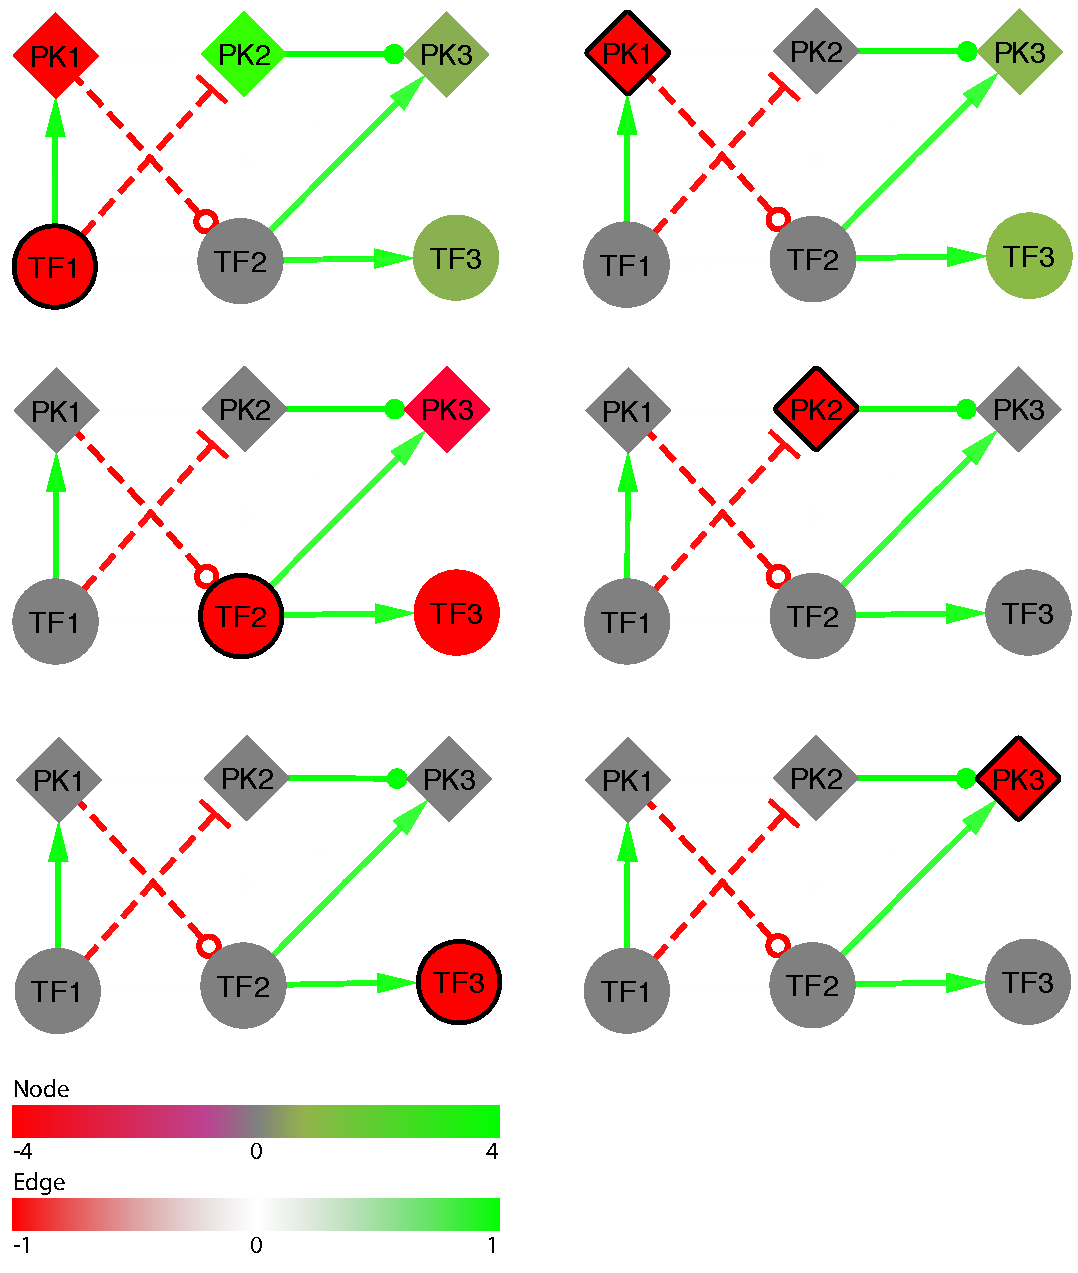
\includegraphics[width=\textwidth]{analysis/fig/gnw.pdf}
\end{subfigure}
\caption{\textbf{DAG node value simulation.} Simple iterative simulation~(a), and extended GeneNetWeaver~(b). LogFC node values. \textcolor{black}{black border} = gene deletion. Edges: true graph. }
\label{fig:dag_data}
\end{figure}

% Two different methods of node value simulation was applied, with the resulting node values indicating with node coloring in~\autoref{fig:dag_data}, where the edges are simply showing the true graph from~\autoref{fig:dag}. The first method is using the inference equations in the simple iterative simulation described in~\autoref{sec:prim}. The second method is applying the GeneNetWeaver kinase extension~(\autoref{sec:gnw_extension}), which is the more realistic simulation approach applying nonlinear gene regulation mechanisms.



% We see how PK regulatory interactions are not directly observed but still detectable through a regulated transcription factor. We also see that the node values are less pronounced when simulated using the GNW extension but otherwise identical in this simple example. Both methods are displaying node values that intuitively would be expected for each given knockout.
\end{column}
\end{columns}
\end{frame}

\begin{frame}{Directed acyclic graph - Inference}

% The $\boldsymbol{e}$-minimization method of edge inference is compared to the original edge inference method LLC~(\autoref{sec:eberhardt}) by using each for edge inference on the simulated node values. The inferred edges on node values simulated using either the simple method or GNW extension are shown in~\autoref{fig:dag_infer}.


\begin{figure}[ht]
\centering
\begin{subfigure}[b]{0.23\textwidth}\centering\caption{}
\includegraphics[width=\textwidth]{analysis/fig/weight.pdf}\label{fig:dag_infer.a}
\end{subfigure}
\hfill
\begin{subfigure}[b]{0.23\textwidth}\centering\caption{}
\includegraphics[width=\textwidth]{analysis/fig/gnwweight.pdf}
\end{subfigure}
\hfill
\begin{subfigure}[b]{0.23\textwidth}\centering\caption{}
\includegraphics[width=\textwidth]{analysis/fig/B.pdf}\label{fig:dag_infer.c}
\end{subfigure}
\hfill
\begin{subfigure}[b]{0.23\textwidth}\centering\caption{}
\includegraphics[width=\textwidth]{analysis/fig/gnwB.pdf}
\end{subfigure}
\vskip\baselineskip
\begin{subfigure}[b]{0.25\textwidth}\centering
\includegraphics[width=\textwidth]{analysis/fig/edge_legend.pdf}
\end{subfigure}
\caption{\textbf{DAG edge inference.}  $\boldsymbol{e}$-minimization~(a,b), and LLC~(c,d). On simple iterative simulation~(a,c), and GeneNetWeaver kinase extension~(b,d).}
\label{fig:dag_infer}
\end{figure}
$\boldsymbol{e}$-minimization captures indirectness, LLC does not
% We see that LLC correctly predicts the TF edges, which are directly influencing node values, but does not capture any edges from the protein kinases, which are indirectly affecting node values~\autoref{fig:dag_infer.c}. We further see that the $\boldsymbol{e}$-minimization method captures all detectable edges~\autoref{fig:dag_infer.a}. The PK edge from $\text{PK}_2$ to $\text{PK}_3$ is undetectable since $\text{PK}_3$ does not regulate anything. For node values simulated with GNW extension it is the same observations, although some edges appear weaker, which can make them harder to detect in noisy data. However, since edge inference is a boolean classification problem, their weakness is not an issue as long as the edge value is above the threshold used for edge detection.


\end{frame}

\begin{frame}{Cyclic graphs}
\label{sec:toy}
\begin{columns}
\begin{column}{0.4\textwidth}
% We now add cycles to the DAG from before~(\autoref{sec:dag}). The edges are also given randomly selected values in range $[-1,1]$~(\autoref{fig:toy}).
\begin{figure}[ht]
    \centering
    \includegraphics[width=0.7\textwidth]{analysis/fig/toy.pdf}
    \caption{\textbf{Directed cyclic networks.} \textcolor{blue}{blue} = edges added onto DAG. Multiple values: four separate graphs each assigned one of the four values. }
    \label{fig:toy}
\end{figure}
% Four separate graphs are tested to analyse the balance between predicting that an edge is present from a protein kinase to a transcription factor or that the observed effect is mediated through another protein kinase.

\vskip2\baselineskip

$\pk_2\rightarrow\pk_3$ is favored over $\pk_2\rightarrow\tf_{}$ when increasing $\pk_3\rightarrow\tf_{}$
\end{column}

\begin{column}{0.6\textwidth}
\begin{figure}[ht]
\centering
\begin{subfigure}[b]{0.4\textwidth}\centering\caption{}
\includegraphics[width=0.8\textwidth]{analysis/fig/cyclic_2.pdf}\label{fig:toy_infer.a}
\end{subfigure}
\quad
\begin{subfigure}[b]{0.4\textwidth}\centering\caption{}
\includegraphics[width=0.8\textwidth]{analysis/fig/cyclic_3.pdf}\label{fig:toy_infer.b}
\end{subfigure}
\vskip\baselineskip
\begin{subfigure}[b]{0.4\textwidth}\centering\caption{}
\includegraphics[width=0.8\textwidth]{analysis/fig/cyclic_4.pdf}\label{fig:toy_infer.c}
\end{subfigure}
\quad
\begin{subfigure}[b]{0.4\textwidth}\centering\caption{}
\includegraphics[width=0.8\textwidth]{analysis/fig/cyclic_5.pdf}\label{fig:toy_infer.d}
\end{subfigure}
\vskip\baselineskip
\begin{subfigure}[b]{0.3\textwidth}\centering
\includegraphics[width=\textwidth]{analysis/fig/edge_legend_cyclic.pdf}
\end{subfigure}
\caption{\textbf{Edge inference.} True $\pk_3\rightarrow\tf_2$ = 0~(\text{a}), -0.6~(\text{b}), -0.3~(c), -0.2~(d). $\boldsymbol{e}$-minimization~($\lambda_T=0.01, \lambda_P=0.01$). Simple simulation. }
\label{fig:toy_infer}
\end{figure}

% Node values were simulated on each of the four graphs with approximate convergence using the simple iterative approach~(\autoref{sec:prim}). Edge values were then inferred using the $\boldsymbol{e}$-minimization method with $\lambda_{TF} = 0.01$ and $\lambda_{PK} = 0.01$~(\autoref{sec:equilibrium_model}). The inferred edges are shown in~\autoref{fig:toy_infer} for each of the four graphs produced from varying a single edge value as indicated in~\autoref{fig:toy}.

% First, the leftmost blue edge in~\autoref{fig:toy} is added to the DAG~(the rightmost blue edge has an edge value of zero). We observe that the inference method now detects the effect of $\pk_2$, but it predicts it is a direct edge to $\tf_1$, rather than an indirect effect mediated by $\pk_3$~(\autoref{fig:toy_infer.a}). This is a rational prediction, given that the node value data would be equivalent in a case where an edge from $\pk_2$ to $\tf_1$ was present, with edge value equal to the product of the true edge values from $\pk_2\rightarrow \pk_3$ and $\pk_3\rightarrow \tf_1$.
\end{column}
\end{columns}
\end{frame}

\begin{frame}{Cyclic graphs - favoring PK$\rightarrow$PK vs. PK$\rightarrow$TF}

% Next, we show that if $\pk_3$ were to have more outgoing edges, in this case directly to $\tf_2$, then the inference will predict the $\pk_2\rightarrow \pk_3$ edge correctly~(\autoref{fig:toy_infer.b}). Even though it is still possible to explain the observed effect from $\pk_2$ to $\tf_1$ and $\tf_2$, it is the favored explanation, that the effect is mediated by a single edge from the protein kinase: $\pk_2 \rightarrow \pk_3$ (option A), rather than needing two edges: $\pk_2 \rightarrow \tf_1$ and $\pk_2 \rightarrow \tf_2$ (option B). This is a result of regularization, where by applying an L1-regularization to all parameters~(edge values), we predict the parameters that explains the data with the smallest possible edge values, which reduces the count of edges and promotes sparsity. 

% The balance between the choice of a PK$\rightarrow$TF edge versus a PK$\rightarrow$PK$\rightarrow$TF path, is based on the smallest sum of absolute edge values for each case. We explore this by reducing the edge value for the rightmost blue edge in~\autoref{fig:toy}. We observe that for small values, option B with two edges, $\pk_2 \rightarrow \tf_1$ and $\pk_2 \rightarrow \tf_2$, will be favorable~(\autoref{fig:toy_infer.d}), and for a certain threshold both option A and B will be equally likely, at which point all paths are inferred to have a combined effect~(\autoref{fig:toy_infer.c}). The threshold is found when the L1-regularization are the same for option A and B, given that $\boldsymbol{e}$ is equal for both options~(\autoref{eq:loss_e}). We formulate the L1-norm cost for all paths from $\pk_2$ in option A and B:
Option A: $\pk_{}\rightarrow\pk_{}$ \\
Option B: $\pk_{}\rightarrow\tf_{}$ \\
Norms differentiating loss for option A and B
\begin{subequations}
\label{eq:toy_l1}
\begin{align}
L1_{\pk_2\rightarrow\pk_3}
&=
|w_{\pk_2\rightarrow\pk_3}^{(\text{A})}|
\\
L1_{\pk_2\rightarrow \{\tf_1,\tf_2\}}
&=
|w_{\pk_2\rightarrow \tf_1}^{(\text{B})}| + |w_{\pk_2\rightarrow \tf_2}^{(\text{B})}|
\label{eq:toy_l1.B}
\end{align}
\end{subequations}


% Superscripts $(\text{A})$ and $(\text{B})$ indicates the option, where a weight parameters $w^{(\text{A})}$ will be nonzero for option A and $w^{(\text{B})}$ nonzero for option B. If the effects from $\pk_2$ to both $\tf_1$ and $\tf_2$ are perfectly captured for option A and B, then the total effects can be written using notation similar to~\autoref{sec:eberhardt}:

Effects from $\pk_2$ to \textcolor{tf}{TFs} are equal for choice A and B
\begin{subequations}
\label{eq:toy_t}
\begin{align}
t(\pk_2 \rightsquigarrow \tf_1)
&=
w_{\pk_2\rightarrow \pk_3}^{(\text{A})} \cdot
t(\pk_3 \rightsquigarrow \tf_1)
=
w_{\pk_2\rightarrow \pk_3}^{(\text{A})} \cdot 
w_{\pk_3\rightarrow \tf_1}
\\
&=
w_{\pk_2\rightarrow \tf_1}^{(\text{B})}
\\
t(\pk_2 \rightsquigarrow \tf_2)
&=
w_{\pk_2\rightarrow \pk_3}^{(\text{A})} \cdot t(\pk_3 \rightsquigarrow \tf_2)
=
w_{\pk_2\rightarrow \pk_3}^{(\text{A})} \cdot w_{\pk_3\rightarrow \tf_2}
\\
&=
w_{\pk_2\rightarrow \tf_2}^{(\text{B})}
\end{align}
\end{subequations}

\end{frame}
\begin{frame}{Cyclic graphs - favoring PK$\rightarrow$PK vs. PK$\rightarrow$TF}


% By summing~\autoref{eq:toy_t} we can formulate $L1_{\pk_2 \rightarrow \pk_3}$:

\begin{subequations}
\begin{align}
|t(\pk_2 \rightsquigarrow \tf_1)| + |t(\pk_2 \rightsquigarrow \tf_2)| &=
|w_{\pk_2\rightarrow \pk_3}^{(\text{A})}|
\left(|w_{\pk_3\rightarrow \tf_1}| + |w_{\pk_3\rightarrow \tf_2}|\right)
\\
&= |w_{\pk_2\rightarrow \tf_1}^{(\text{B})}| + |w_{\pk_2\rightarrow \tf_2}^{(\text{B})}|
\\
\implies
L1_{\pk_2 \rightarrow \pk_3}
&=
\frac
{|w_{\pk_2\rightarrow \tf_1}^{(\text{B})}| + |w_{\pk_2\rightarrow \tf_2}^{(\text{B})}|}
{|w_{\pk_3\rightarrow \tf_1}| + |w_{\pk_3\rightarrow \tf_2}|}
\\
&=
\frac{
L1_{\pk_2\rightarrow\{\tf_1,\tf_2\}}
}{
|w_{\pk_3\rightarrow\tf_1}| + |w_{\pk_3\rightarrow \tf_2}|
}
\end{align}
\end{subequations}

% This means that option A has the lowest L1-norm, and is inferred, when edges from $\pk_3$ sum to more than 1, option B is inferred when they sum to less than 1, and both options are combined when edges from $\pk_3$ sum to 1. It is demonstrated in~\autoref{fig:toy_infer.b}, \ref{fig:toy_infer.c}, and \ref{fig:toy_infer.d}, where the sums are $|-0.7| + |-0.6| = 1.2$, $|-0.7| + |-0.3| = 1.0$, and $|-0.7| + |-0.2| = 0.9$.

Option A favored when $|w_{\pk_3\rightarrow \tf_1}| + |w_{\pk_3\rightarrow \tf_2}| < 1$

General formulations (more norms may be compared):

% So, if the data can be perfectly modeled in either case considered, then for an edge $\text{PK}_j \rightarrow \text{PK}_i$ and for the case of direct edges from $\text{PK}_j$ to each regulated $\text{TF}_k$ the generalized L1-norms will be

\begin{subequations}
\begin{align}
L1_{\text{PK}_j \rightarrow \text{PK}_i}
&=
\frac{
L1_{\text{PK}_j \rightarrow \{\text{TF}_k\}}
}{
\sum_k |t(\text{PK}_i \rightsquigarrow \text{TF}_k)|
}
\\
L1_{\text{PK}_j \rightarrow \{\text{TF}_k\}}
&=
\sum_k |w_{\text{PK}_j \rightarrow \text{TF}_k}|
\end{align}
\end{subequations}

% Where $k$ indexes all TFs that are regulated by $\text{PK}_j$ through a directed path of PKs.

% For a more complicated graph, there can be many other L1-norms that the model will compare, than the two exemplified here.
% In general, applying the L1-regularization indiscriminately on each parameter will make the model favor paths with fewer edges. The smaller the parameters found for a dataset, the rarer PK$\rightarrow$PK edges will be inferred. The parameters will usually be less than 1 since parameters above 1 easily leads to divergence in the model.
\end{frame}
\begin{frame}{Loss function favoring longer cascades}
\label{sec:cascade_loss}
\begin{columns}
\begin{column}{0.65\textwidth}

% Other loss functions can be considered to treat longer cascades more favorably. One idea would be to replace the use of the regularization hyperparameter $\lambda_{PK}$ with a regularization strength for $\text{PK}\rightarrow\text{TF}$ and a smaller one for $\text{PK}\rightarrow\text{PK}$ edges, however this creates loops among the PKs to artificially strengthen the $\text{PK}\rightarrow\text{TF}$ edges~(not shown).

% A solution to consider is replacing the L1-regularization of PK edges with a loss based on a sum of effects $t(\text{PK}_j\rightsquigarrow\text{TF}_i)$ that each PK has through all its cascades. This is done in a similar fashion to the classification of detectable nodes~(\autoref{sec:unobservable}). 

PK edge norm = total effect on TFs
\begin{equation}
\label{eq:pk_effect}
\boldsymbol{l}_{\text{cas}} =
\sum_{k=1}^K {(|W|I_P)^\trans}^k
(I_T \boldsymbol{1} )
\end{equation}

% Here, $|W|$ is used for indication of element-wise absolute values of $W$. $K$ can be found similarly to described in~\autoref{sec:unobservable}, however due to noise in the weights while training it is best to have an upper bound for $K$, which can be chosen conservatively since the only downside to using a too large $K$ is computational cost. $W$ has to be square. If there are more measured genes than knockouts, we use $I_SW$ instead, where $I_S$ is an identity matrix with dimensions $(N_T + N_P) \times N$, and $N$ is the total number of measured genes.

% If $I-(|W|I_P)^\trans$ is invertible, we can get rid of $K$ from~\autoref{eq:pk_effect}, as it was done in~\autoref{sec:unobservable}.
for $K\rightarrow\infty$
\begin{equation}
\boldsymbol{l}_{\text{cas}} =
\left(
\sum_{k=1}^\infty {(|W|I_P)^\trans}^k
\right)
(I_T \boldsymbol{1} )
=
\left(
I-(|W|I_P)^\trans
\right)^{-1}
(I_T \boldsymbol{1} )
\end{equation}

% We define a new loss function that favors longer cascades:

\begin{equation}
\mathcal{L}_\text{cas} =
\sum_{i=1}^N e_i^2 + \lambda_T \sum_{j \in \text{TF}} \sum_{i=1}^N |w_{ij}| + \lambda_P \sum_{i=0}^{N_T + N_P} \left(
\sum_{j \in \text{PK}} |w_{ij}|
+ l_i^{(\text{cas})}
\right)
\label{eq:loss_cas}
\end{equation}

% Here, $\boldsymbol{l}_{\text{cas}}$ and the L1-norm regularization term used in~\autoref{eq:loss_e} are summed, where  $l_i^{(\text{cas})}$ is the $i$-th element of $\boldsymbol{l}_\text{cas}$.

\end{column}
\begin{column}{0.35\textwidth}
\begin{figure}[ht]
\centering
\begin{subfigure}[b]{0.7\textwidth}\centering
\includegraphics[width=\textwidth]{analysis/fig/cyclic_4_cas.pdf}
\end{subfigure}
\vskip\baselineskip
\begin{subfigure}[b]{0.5\textwidth}\centering
\includegraphics[width=\textwidth]{analysis/fig/edge_legend_cyclic.pdf}
\end{subfigure}
\caption{\textbf{Correcting inference.} Inference from~fig.~\ref{fig:toy_infer.c} using $\mathcal{L}_\text{cas}$~(eq.~\ref{eq:loss_cas}) instead of $\mathcal{L}_{\boldsymbol{e}}$~(eq.~\ref{eq:loss_e}).
$\lambda_T=0.01$, $\lambda_P=0.01$. }
\label{fig:toy_cas}
\end{figure}

% The loss function was tested for edge inference otherwise identical to the procedure for~\autoref{fig:toy_infer.c}, for instance instance by using $\lambda_T=0.01$ and $\lambda_P=0.01$ as before. The inferred edge values are shown in~\autoref{fig:toy_cas}. We see that the change in loss function has corrected the inference to favor the $\pk_2\rightarrow\pk_3$ edge, which has been referred to as option A.

% The remaining work in this section describes inference attempts using standard L1-regularization. $\mathcal{L}_\text{cas}$ has yet to be tested for possibilities of improving performance on larger networks.
\end{column}
\end{columns}
\end{frame}

\begin{frame}{Edge inference on DREAM networks - 10 nodes}
\label{sec:dream_results}
\begin{columns}
\begin{column}{0.4\textwidth}
% The DREAM data goldstandards for the five 10-node graphs were used for simulation of node values using the simple iteration method~(\autoref{sec:prim}), after randomly assigning uniform edge strengths in range~$[-1,1]$.

\begin{figure}[ht]
    \centering
    \includegraphics[width=\textwidth]{analysis/fig/edge_cor_10.pdf}
    \caption{\textbf{Predicted vs. true edge values.} 5 10-node networks. Simple simulation. }
    \label{fig:edge_value_cor_10}
\end{figure}

% The resulting inferred edge values for a single edge inference attempt on each graph are compared to the true edge values~(\autoref{fig:edge_value_cor_10}). There are three undetectable edges for the five graphs. They are included in this plot and all have a score of zero. The points along the line \texttt{score}=\texttt{true} are edges where the weight~(score) accurately predicts the true edge strength used for node value simulation. A few outlier protein kinase edges can be seen as being misclassified. Most values are found in the point (0,0) which are all non-edges correctly classfied as non-edges (true negatives). The purpose of the plot is to show that for very simple cases the edges are not only found, but their exact edge value is also inferred. It also shows that there is 1 false positive and 1 false negative of the 15 detectable PK edges, and that inference on TF edges are perfect in this simple example.
\begin{itemize}
    \item Predicted edge values accurate to truth
    \item LLC fails for kinases
\end{itemize}
\end{column}
\begin{column}{0.6\textwidth}

\begin{figure}[ht]
\centering
\begin{subfigure}[b]{0.49\textwidth}\centering\caption{}
\includegraphics[width=\textwidth]{analysis/fig/roc_pk_10.pdf}
\end{subfigure}
\hfill
\begin{subfigure}[b]{0.49\textwidth}\centering\caption{}
\includegraphics[width=\textwidth]{analysis/fig/roc_pk_llc_10.pdf}
\end{subfigure}
\caption{\textbf{ROC curves for 5 10-node networks.} $\boldsymbol{e}$-minimization~(a) and LLC~\cite{EberhardtLLC}~(b) on PK edges. neg: inference of negative edges, pos: positive, abs: ignoring sign. AUCs are micro averaged.}
\label{fig:roc_pk_10}
\end{figure}

% The inference can also be described with ROC curves for outgoing PK edges in each individual graph~(\autoref{fig:roc_pk_10}). Inference of the presence or absence of edges from transcription factors to genes were perfect on this simple simulation~(AUC=1). For protein kinases the inference is less trivial, as we see that AUCs drops below perfect scores. Note that most curves are perfect, and that the ones not following the path (0,0)$\rightarrow$(0,1)$\rightarrow$(1,1) are a minority. This is also apparent from the AUC scores, which are close to perfect. The ROC curves are also shown for inference performed using the LLC method~\cite{EberhardtLLC}. Since it infers linear direct causal interactions and it fails to classify presence and absence of outgoing PK edges based on their indirect effects on the observed node values.
\end{column}
\end{columns}
\end{frame}

\begin{frame}{Edge inference on DREAM networks - 100 nodes}
% This comparison is biased towards the equilibrium method since the data simulation is performed with the same equations that are used for the $\boldsymbol{e}$-minimization inference, so to increase realism and fairness of performance testing we move on to the larger 100-node graphs where we will use the more realistic GeneNetWeaver kinase extension code for simulation of observable node values.
\begin{figure}[ht]
\centering
\begin{subfigure}[b]{0.24\textwidth}\centering\caption{}
\includegraphics[width=\textwidth]{analysis/fig/roc_pk_prim.pdf}
\end{subfigure}
\hfill
\begin{subfigure}[b]{0.24\textwidth}\centering\caption{}
\includegraphics[width=\textwidth]{analysis/fig/roc_pk_prim_B.pdf}
\end{subfigure}
\hfill
\begin{subfigure}[b]{0.24\textwidth}\centering\caption{}
\includegraphics[width=\textwidth]{analysis/fig/roc_pk_gnw_pos.pdf}\label{fig:micro_average.c}
\end{subfigure}
\hfill
\begin{subfigure}[b]{0.24\textwidth}\centering\caption{}
\includegraphics[width=\textwidth]{analysis/fig/roc_pk_gnw.pdf}\label{fig:micro_average.d}
\end{subfigure}
\caption{\textbf{ROC curves for PK edge inference.} $\boldsymbol{e}$-minimization~(a,c,d) and $B$-method~(b). Simple simulation~(a,b), and GeneNetWeaver extension~(c,d). True PK edges all positive~(c) or signed~(d). neg: inference on negative edges. pos: positive. abs: ignoring sign. avg: score = avg. $w$ from 20 runs. avg/std: score = avg./std. $w$, other: score = $w$. }
\label{fig:micro_average}
\end{figure}
$\ge 80 \%$ most prominent edges inferred perfectly
% Edge inference was tested on the five 100-node graphs from DREAM4. The simulations were either performed using the simple iteration method~(\autoref{sec:prim}) or the GeneNetWeaver kinase extension method~(\autoref{sec:gnw_extension}). TF inference was almost perfect with AUC=0.992 for detection of presence or absence of edge, which can be seen in the appendix~(\autoref{fig:gnw_each.a}). The ROC curves, shown in~\autoref{fig:micro_average}, are evaluated on comparisons of inferred and true edges, combined of all five graphs~(microaverage). Individual graphs for individual runs can be seen in~\autoref{app:roc} with equivalent AUC scores.
% Data created with the GNW extension were either simulated where true outgoing PK edges were restricted to a uniform distribution with range~$[0,1]$, or without sign restriction. ROC curves for performance of inference on the former is in~\autoref{fig:micro_average.c}, and the latter in~\autoref{fig:micro_average.d}. The reason for restricting the kinase interaction to positive values are based on the kinase model of regulation~(\autoref{sec:gnw_extension}), which builds on a model of phosphorylation regulation involving only protein kinases with positive interactions~(\autoref{sec:Heinrich}). From the ROC curves it is clear that allowing negative outgoing protein kinase edges does not seem to worsen performance of inference. The negative outgoing protein kinase edges can be seen as a dephosphorylation of the target protein, since $\phi_i$ and $y_i$ from~\autoref{sec:gnw_extension} describes phosphorylation values, and not a general activity concept. It shows that the simulation code and method is robust in allowing for dephosphorylation interactions between specific proteins, rather than only as a background decay~$\lambda_i^{(\text{Phos})}$, since the simulations managed to reach approximate convergence and produce similar inference performance to the trials with sign restriction. Phosphatases are often considered as a background effect to let signals decay, due to their low interaction specificity compared to protein kinases. In spite of this, it is useful that direct dephosphorylation can be simulated and inferred since some of the knockouts in the RNA data are phosphatases~(\autoref{sec:yeast_data}).


% The ROC curves shows a quantitative measure of performance but does not show a final inferred network. To select specific edges we choose a threshold. The threshold was chosen as 0.01 which corresponds to approximately accepting 50\% of inferred PK edges across the five graphs with the highet scores, which corresponds to a cutoff at TPR=0.5 in~\autoref{fig:micro_average.c}. The threshold was applied to all five graphs for all edge types, although different threshold for each were found to be optimal. The inferred edges are shown on the graphs~(\autoref{fig:dream_100_infer}). Activation and repression is not indicated, which is the sign of edges from transcription factors. Edges from protein kinases are all activating as per the restriction to elicit phosphorylation and not dephosphorylation. Kinases not connected to any nodes are included next to each graph. The unconnected kinases are the undetectable kinases. The count of undetectable kinases for each graph is 30 minus the "detectable PK nodes" counts listed in~\autoref{tab:dream_data}, since each graph were initially assigned 30 kinases.

% From the plots we get an impression of the intricacy arising from less than 100 nodes. We see that edges inferred can often be trusted, detects many of the true edges, and that false positives for PK edges arises in situations where there would be ambiguity in what regulation to expect, given only the relative gene expressions. An example is the $\text{PK}_{14}\rightarrow\text{PK}_{29}$ edge at the top-right of net 100.4.
\end{frame}

\begin{frame}{Edge inference on DREAM networks - 100 nodes}
\begin{figure}[ht]
    \centering
    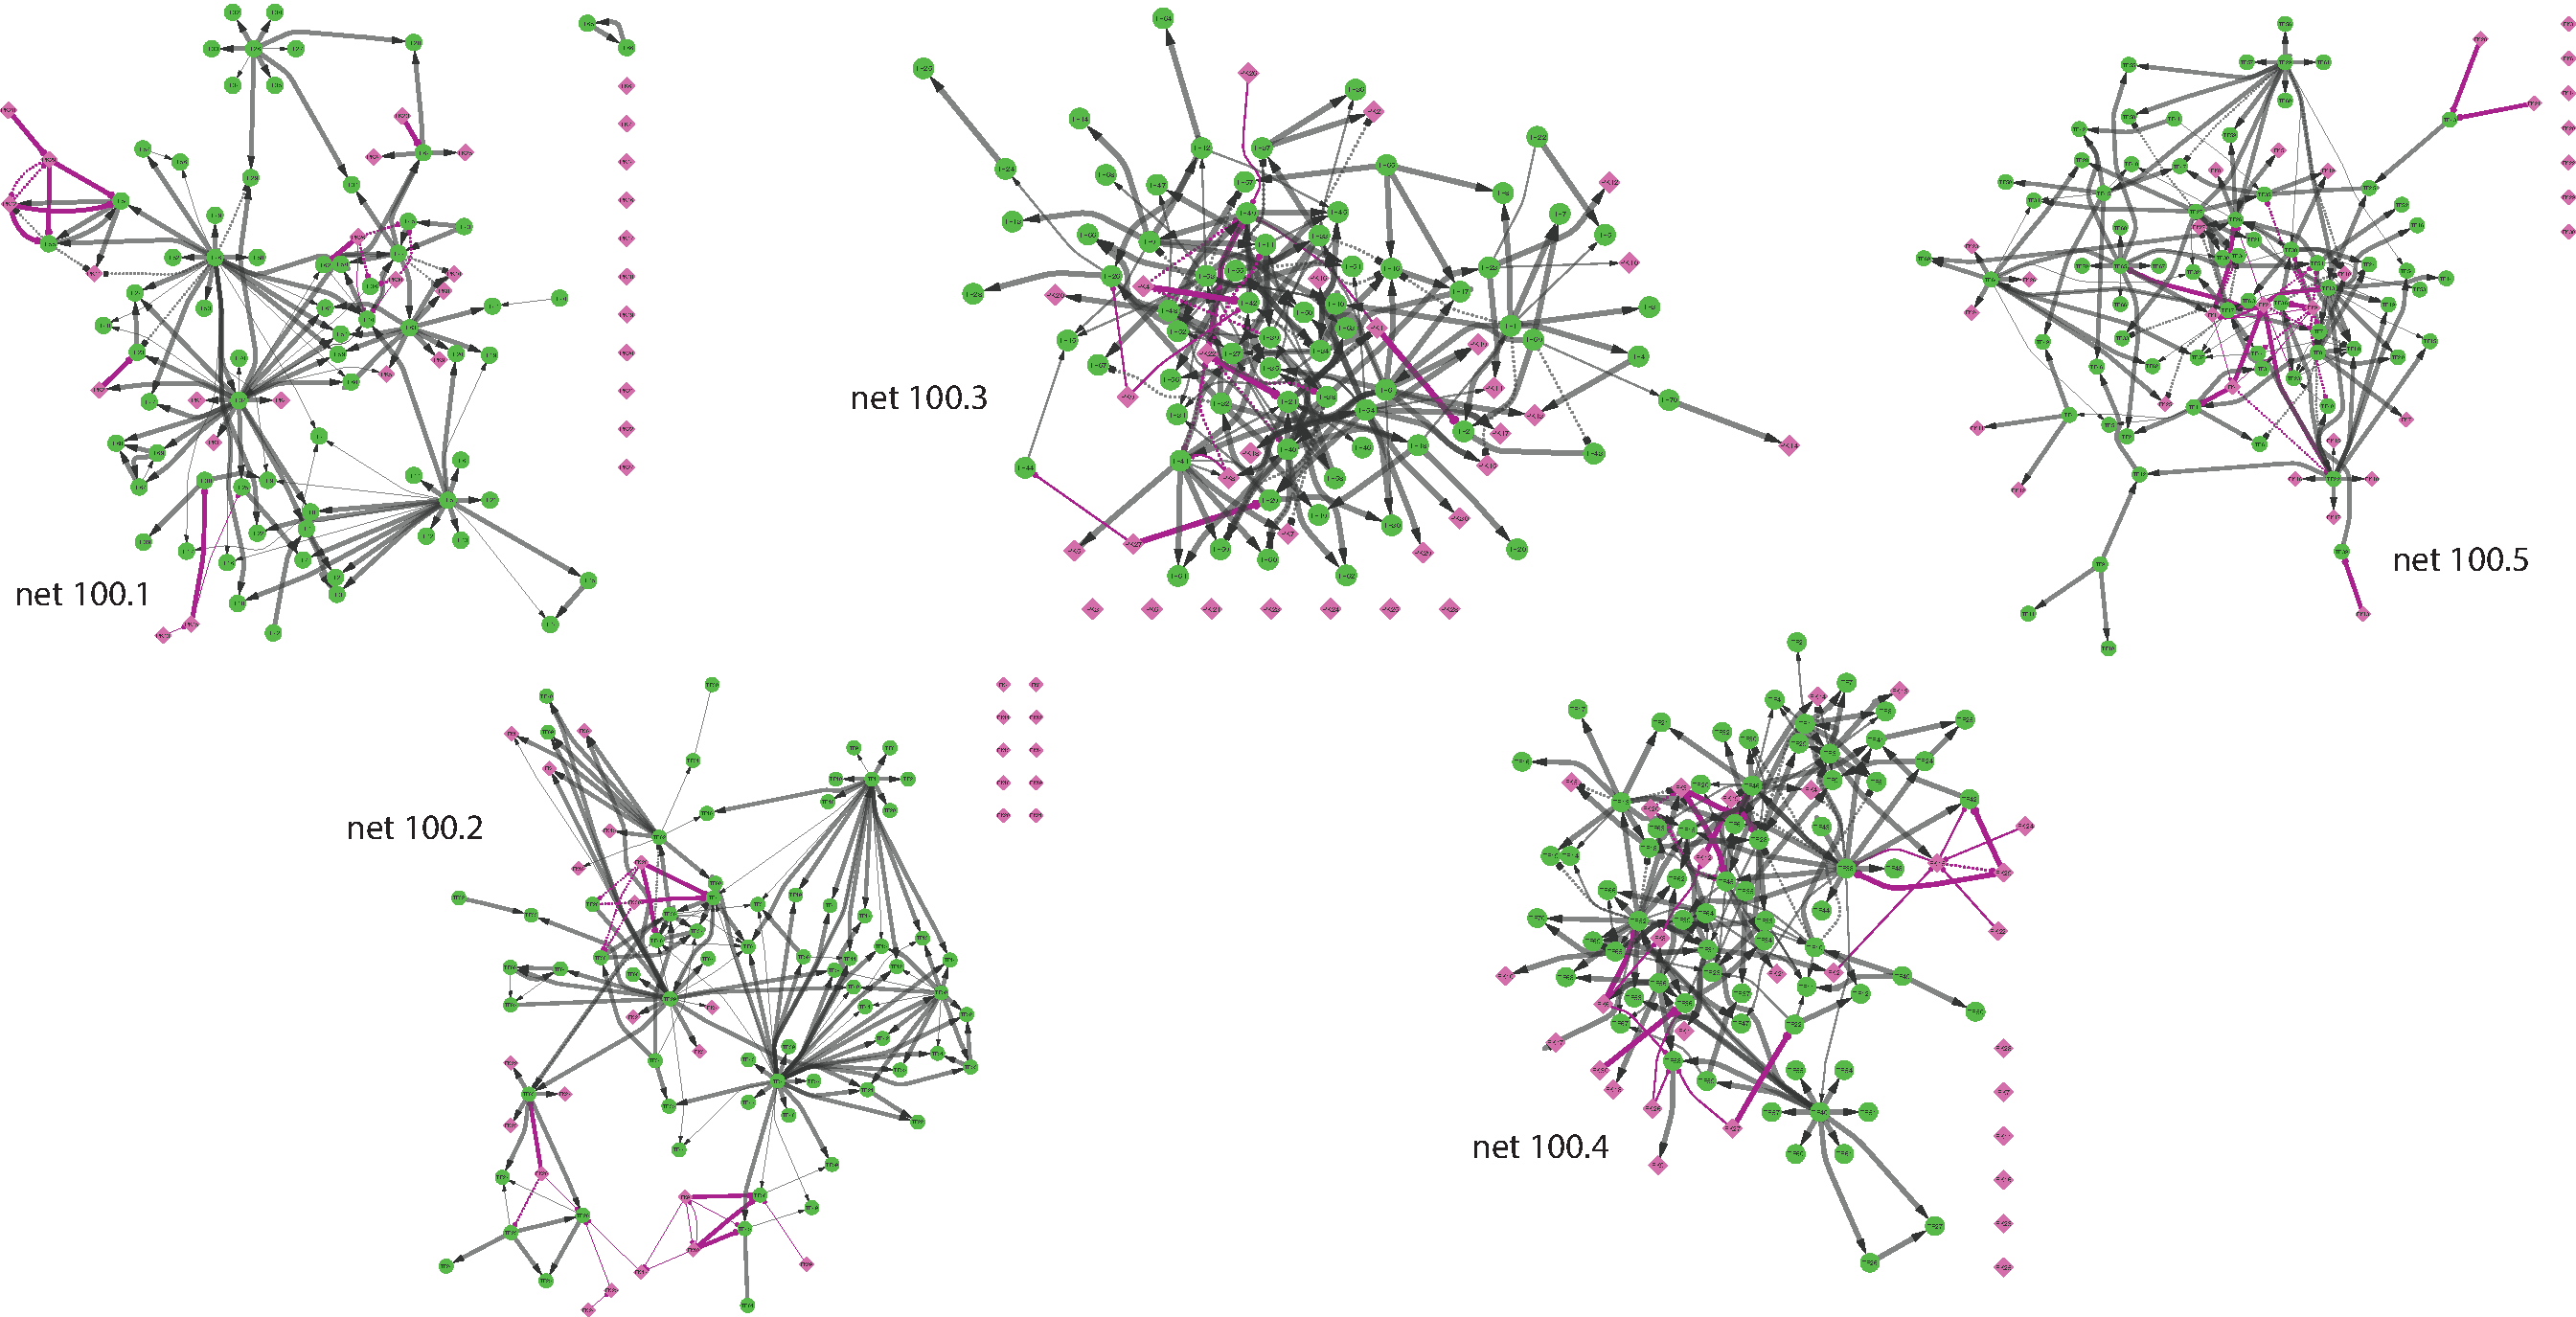
\includegraphics[width=.93\textwidth]{analysis/fig/dream100_infer_pres.pdf}
    \caption{\textbf{Inferred edges of 5 100-node networks.} Edge inferred from single $\boldsymbol{e}$-minimization when $w>0.01$. \textbf{Thick line} = TP, thin = FN, dotted = FP, none = TN. \textcolor{gray}{Dim line} = TF edge, \textcolor{pk!50!magenta}{magenta} = PK edge. }
    \label{fig:dream_100_infer}
\end{figure}
\end{frame}


% \begin{frame}{Protein kinase interaction inference on yeast data}
% \label{sec:yeast_results}
% \begin{columns}
% \newcommand\histwidth{0.36\textwidth}
% \begin{column}{0.5\textwidth}
% % The TF$\rightarrow$gene edges from the data are assumed to be the full set of transcription factors and the signs of their interactions are also enforced for edges where it is known in the Yeastract dataset, as described in~\autoref{sec:data_preprocess}. The inference is performed on edges with protein kinases as source node. For TFs, the model predicts edge strengths, and, in cases with unknown sign, it predicts the sign of interaction.


% \begin{figure}[ht]
% \centering
% \begin{subfigure}[b]{\histwidth}\centering\caption{}
% \includegraphics[width=\textwidth]{analysis/fig/hist_pk-tf_high_single.pdf}\label{fig:yeast_hist_single.a}
% \end{subfigure}
% \quad
% \begin{subfigure}[b]{\histwidth}\centering\caption{}
% \includegraphics[width=\textwidth]{analysis/fig/hist_pk-pk_high_single.pdf}\label{fig:yeast_hist_single.b}
% \end{subfigure}
% % \vskip\baselineskip
% \begin{subfigure}[b]{\histwidth}\centering\caption{}
% \includegraphics[width=\textwidth]{analysis/fig/hist_pk-tf_single.pdf}\label{fig:yeast_hist_single.c}
% \end{subfigure}
% \quad
% \begin{subfigure}[b]{\histwidth}\centering\caption{}
% \includegraphics[width=\textwidth]{analysis/fig/hist_pk-pk_single.pdf}\label{fig:yeast_hist_single.d}
% \end{subfigure}
% \caption{\textbf{PK edge inference on yeast.} High quality edges~(a,b) and unknown/less likely edges~(c,d). }
% \label{fig:yeast_hist_single}
% \end{figure}

% % Edge inference was attempted on the RNA log fold-change data~(\autoref{sec:yeast_data}). Densities of scores for edges from different datasets can be seen in~\autoref{fig:yeast_hist_single} for a single attempt at minimizing~$\boldsymbol{e}$ where the score is the absolute weight value, and in~\autoref{fig:yeast_hist_avgstd} normalized scores where multiple individual attempts at minimizing~$\boldsymbol{e}$ were performed and normalized so that the scores are average weight values divided by the empirical standard deviation observed for each. The LLC method was used for comparison which can be found in~\autoref{fig:yeast_hist_llc} in the appendix, where it can be seen that there is no clear difference between datasets. Inference was also attempted by letting the score of an edge be the average weight from multiple individual minimization of~$\boldsymbol{e}$, with similar results to the normalized attempt~(\autoref{fig:yeast_hist_avg}). All density plots are split into subplots for datasets where we expect all edges should be true edges and the low confidence datasets biogrid and the category "unknown" which holds all entries of the adjacency matrix where an edge is possible, yet not found in any of the other datasets.

% \end{column}
% \begin{column}{0.5\textwidth}
% \begin{figure}[ht]
% \centering
% \begin{subfigure}[b]{\histwidth}\centering\caption{}
% \includegraphics[width=\textwidth]{analysis/fig/hist_pk-tf_high_avgstd.pdf}
% \end{subfigure}
% \quad
% \begin{subfigure}[b]{\histwidth}\centering\caption{}
% \includegraphics[width=\textwidth]{analysis/fig/hist_pk-pk_high_avgstd.pdf}
% \end{subfigure}
% % \vskip\baselineskip
% \begin{subfigure}[b]{\histwidth}\centering\caption{}
% \includegraphics[width=\textwidth]{analysis/fig/hist_pk-tf_avgstd.pdf}
% \end{subfigure}
% \quad
% \begin{subfigure}[b]{\histwidth}\centering\caption{}
% \includegraphics[width=\textwidth]{analysis/fig/hist_pk-pk_avgstd.pdf}
% \end{subfigure}
% \caption{\textbf{Normalized PK edge inference on yeast.} High quality edges~(a,b) and unknown/less likely edges~(c,d). }
% \label{fig:yeast_hist_avgstd}
% \end{figure}
% \end{column}
% % We observe that two peaks appear in the density plots, at around score=\num{1e-4} and score=\num{3e-2} for~\autoref{fig:yeast_hist_single} as well as score=\num{1e-1} and score=\num{1e+1} for~\autoref{fig:yeast_hist_avgstd}. The peaks are visible for PK$\rightarrow$TF edges but PK$\rightarrow$PK edge inference is not clearly divided. The peaks can be useful for categorizing edges as present or absent, with the peak at lower score classifying absence of edges and the other indicating presence. We see that for datasets with edges assumed to be known, there are higher densities for peaks at higher scores~(\autoref{fig:yeast_hist_single.a}). This is especially seen for Fasolo~et~al. data but barely for EMAP data~\autoref{sec:fiedler_data}. The opposite is the case for datasets where the edge presence and absence are unknown~(\autoref{fig:yeast_hist_single.c}). Since the adjacency matrices should overall be sparse there would be many non-edges. 
% \end{columns}
% \end{frame}

\begin{frame}{Inference performance}
\begin{columns}
\begin{column}{0.2\textwidth}
(A) Simulated data \\
(B-C) Yeast data
\begin{itemize}
    \item No negative examples
    \item Few datapoints
\end{itemize}
\end{column}

\begin{column}{0.8\textwidth}
\begin{figure}[ht]
    \centering
    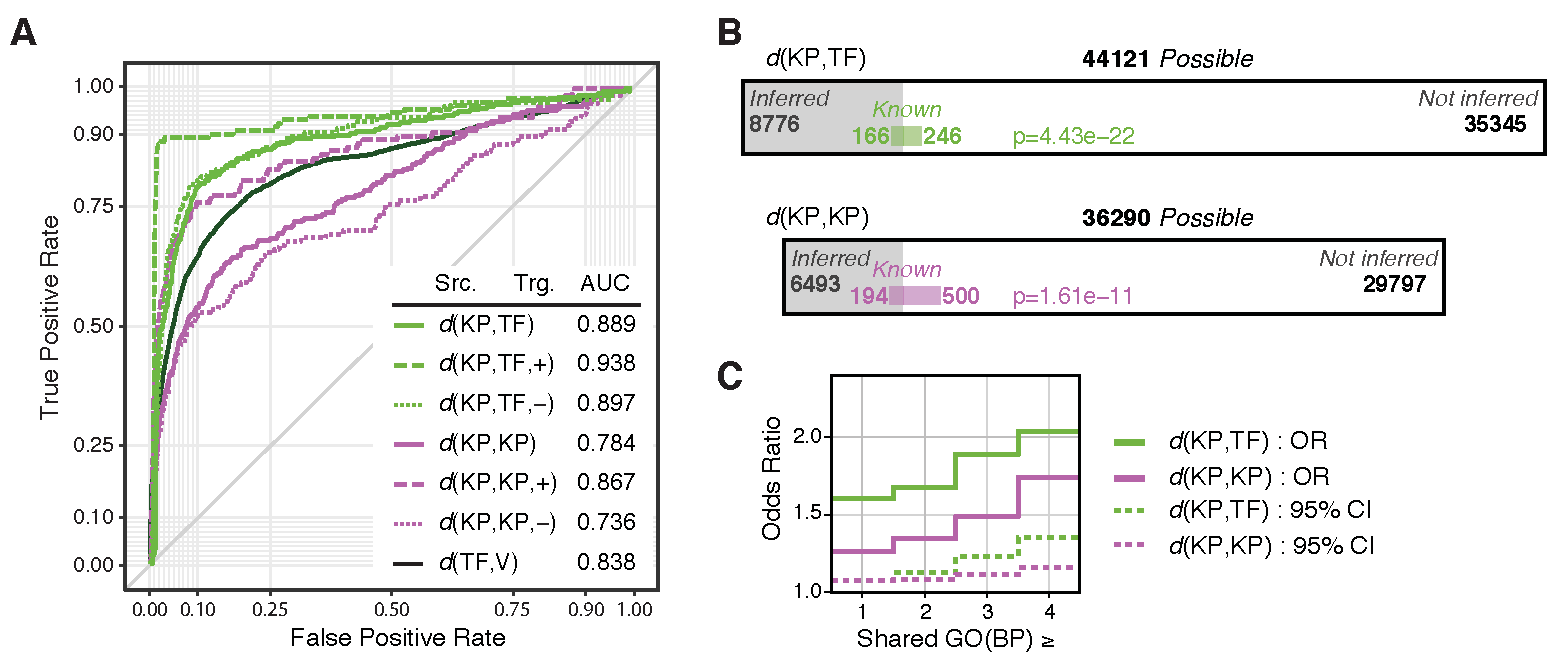
\includegraphics[width=0.85\textwidth]{analysis/fig/Fig3.pdf}
    \caption{\textbf{Performance on simulated and yeast data.} \\  }
    \label{fig:minimum_performance}
\end{figure}
% Since the datasets for evaluation of performance only provides examples of presence of edges~(positive examples), we cannot directly evaluate balance between accuracy, specificity, etc. for the model. By using all possible edges not in a dataset of known edges we get a minimum performance where many of the datapoints used as negatives are in fact positives~(\autoref{fig:minimum_performance}). The Fiedler dataset with PK$\rightarrow$TF edges is included, since it was the single dataset with best performance. We see that PK$\rightarrow$PK edges from any dataset has no noticeably higher scoring than edges not in the dataset. PK$\rightarrow$TF edges from the datasets with known edges has a clear but small overrepresentation as larger scoring edges compared to other possible edges.
\end{column}
\end{columns}
\end{frame}



